
% File acl2020.tex
%
%% Based on the style files for ACL 2020, which were
%% Based on the style files for ACL 2018, NAACL 2018/19, which were
%% Based on the style files for ACL-2015, with some improvements
%  taken from the NAACL-2016 style
%% Based on the style files for ACL-2014, which were, in turn,
%% based on ACL-2013, ACL-2012, ACL-2011, ACL-2010, ACL-IJCNLP-2009,
%% EACL-2009, IJCNLP-2008...
%% Based on the style files for EACL 2006 by 
%%e.agirre@ehu.es or Sergi.Balari@uab.es
%% and that of ACL 08 by Joakim Nivre and Noah Smith

\documentclass[11pt,a4paper]{article}
\usepackage[hyperref]{acl2020}
\usepackage{times}
\usepackage{graphicx}
\usepackage{latexsym}
\usepackage{float}
\usepackage{placeins}
\usepackage{booktabs}
\renewcommand{\UrlFont}{\ttfamily\small}

% This is not strictly necessary, and may be commented out,
% but it will improve the layout of the manuscript,
% and will typically save some space.
\usepackage{microtype}

\aclfinalcopy % Uncomment this line for the final submission
%\def\aclpaperid{***} %  Enter the acl Paper ID here

%\setlength\titlebox{5cm}
% You can expand the titlebox if you need extra space
% to show all the authors. Please do not make the titlebox
% smaller than 5cm (the original size); we will check this
% in the camera-ready version and ask you to change it back.

\newcommand\BibTeX{B\textsc{ib}\TeX}

%%%%%%%%%%%%%%%%%%%%%%%%%%%%%%%%%%%%%%%%%%%%%%%%%%%%

\title{Hw2: Language Modeling of Different Corpuses by Domain and Timeframe}

\author{Sam Showalter \\
  University of California, Irvine \ (showalte) \\  
  Kaggle: Sam Showalter \\
\texttt{showalte@uci.edu}} 

\date{}

%%%%%%%%%%%%%%%%%%%%%%%%%%%%%%%%%%%%%%%%%%%%%%%%%%%%

\begin{document}
\maketitle
\begin{abstract}
  SOMETHING \cite{chen1999empirical}
\end{abstract}


%%%%%%%%%%%%%%%%%%%%%%%%%%%%%%%%%%%%%%%%%%%%%%%%%%%%
% Introduction
%%%%%%%%%%%%%%%%%%%%%%%%%%%%%%%%%%%%%%%%%%%%%%%%%%%%
\section{Related Work: Language Model Implementations}

SOMETHING


%%%%%%%%%%%%%%%%%%%%%%%%%%%%%%%%%%%%%%%%%%%%%%%%%%%%
% Experimental setup
%%%%%%%%%%%%%%%%%%%%%%%%%%%%%%%%%%%%%%%%%%%%%%%%%%%%
\section{Experimental Setup}%
\label{sec:experimental_setup}

SOMETHING


%%%%%%%%%%%%%%%%%%%%%%%%%%%%%%%%%%%%%%%%%%%%%%%%%%%%
% Analysis of in and out of domain text
%%%%%%%%%%%%%%%%%%%%%%%%%%%%%%%%%%%%%%%%%%%%%%%%%%%%
\section{Hyperparameter Tuning}%
\label{sec:hyperparam_tuning}

%%%%%%%%%%%%%%%%%%%%%%%%%%%%%%%%%%%%%%%%%%%%%%%%%%%%
% Token dimensionality exploration
%%%%%%%%%%%%%%%%%%%%%%%%%%%%%%%%%%%%%%%%%%%%%%%%%%%%
\begin{figure*}[htpb]
  \centering
  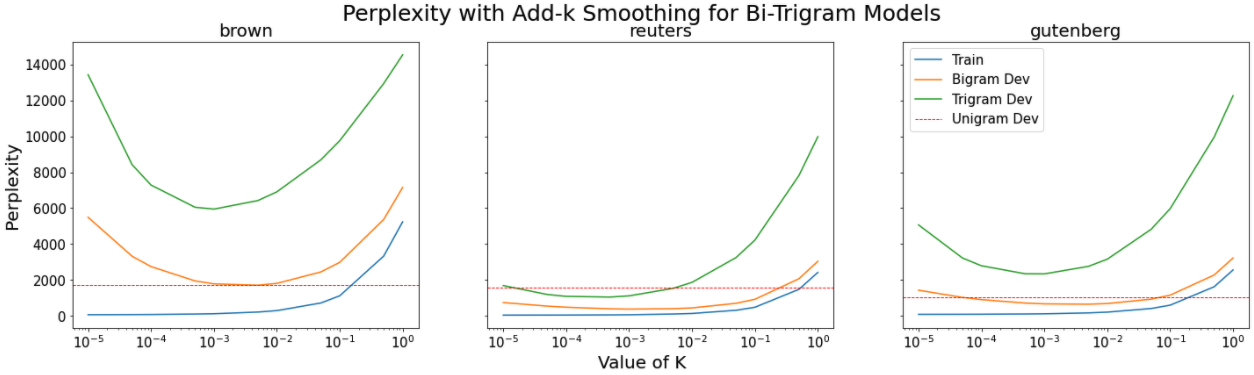
\includegraphics[width=1\linewidth]{imgs/smooth_all.png}
  \caption{Train and dev-set perplexity for bi- and tri-gram 
  language models with vary k in add-k smoothing. A k=1 represents
Laplacian smoothing while dropping k represents weakening the Dirichlet 
prior based on the data. Referenced is dev-set perplexity for unigram models.}
  \label{fig:imgs/smooth_all}
  % \vspace{-10pt}
\end{figure*}
%%%%%%%%%%%%%%%%%%%%%%%%%%%%%%%%%%%%%%%%%%%%%%%%%%%%

%%%%%%%%%%%%%%%%%%%%%%%%%%%%%%%%%%%%%%%%%%%%%%%%%%%%
% Figure of backoff
%%%%%%%%%%%%%%%%%%%%%%%%%%%%%%%%%%%%%%%%%%%%%%%%%%%%
\begin{figure*}[htpb]
  \centering
  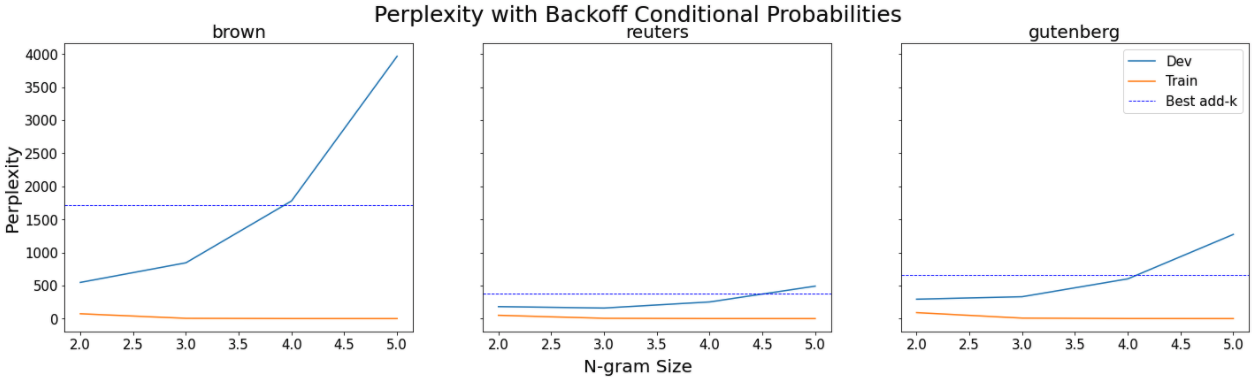
\includegraphics[width=1\linewidth]{imgs/backoff.png}
  \caption{Dev-set perplexity across corpuses with stupid backoff
  smoothing implemented with $\lambda=0.4$ and varing number of
  context sizes (n-gram length). Referenced is current best 
performance from add-k smoothing (dotted).}
  \label{fig:backoff}
\end{figure*}


%%%%%%%%%%%%%%%%%%%%%%%%%%%%%%%%%%%%%%%%%%%%%%%%%%%%
% In-domain Analysis - Empirical
%%%%%%%%%%%%%%%%%%%%%%%%%%%%%%%%%%%%%%%%%%%%%%%%%%%%

\subsection{In-Domain Text Analysis: Empirical}%
\label{sec:in_domain_text_analysis_empirical}


%%%%%%%%%%%%%%%%%%%%%%%%%%%%%%%%%%%%%%%%%%%%%%%%%%%%
% Table for in-domain analysis
%%%%%%%%%%%%%%%%%%%%%%%%%%%%%%%%%%%%%%%%%%%%%%%%%%%%
\begin{table}
\begin{tabular}{llll}
\hline
         & brown       & reuters     & gutenberg   \\
\hline
 uni. & 1514 / 1758 & 1467 / 1577 & 981 / 1036  \\
 add-k   & 128 / 1822  & 72 / 378    & 124 / 650   \\
 b-off & 75 / 559    & 51 / 180    & 92 / 285    \\
\hline
\end{tabular}
\caption{Hyperparameter tuning results. Dev-set perplexity across
all three corpuses with different smoothing. add-k and backoff (b-off) 
running optimal k=0.01 and n=2 for ngram models}
\label{table:hyperparameter}
\end{table}


%%%%%%%%%%%%%%%%%%%%%%%%%%%%%%%%%%%%%%%%%%%%%%%%%%%%
% Out-of-domain Analysis - Empirical
%%%%%%%%%%%%%%%%%%%%%%%%%%%%%%%%%%%%%%%%%%%%%%%%%%%%

\subsection{Out-of-Domain Text Analysis: Empirical}%
\label{sec:out_domain_text_analysis_empirical}


%%%%%%%%%%%%%%%%%%%%%%%%%%%%%%%%%%%%%%%%%%%%%%%%%%%%
% Test perplexity for backoff model
%%%%%%%%%%%%%%%%%%%%%%%%%%%%%%%%%%%%%%%%%%%%%%%%%%%%
\begin{table}[h]
\begin{tabular}{lrrr}
\hline
           &   brown &   reuters &   gutenberg \\
\hline
 brown     &  558.59 &  2118.33  &     840.811 \\
 reuters   & 1500.02 &   180.312 &    2159.68  \\
 gutenberg & 1098.51 &  4240.6   &     285.342 \\
\hline
\end{tabular}
\caption{Test set perpexlity for each language model with
  stupid backoff smoothing applied. Each model is applied to 
every corpus.}
\label{table:backoff_test_perp}
\end{table}

%%%%%%%%%%%%%%%%%%%%%%%%%%%%%%%%%%%%%%%%%%%%%%%%%%%%
% Out-of-domain Analysis - Qualitative
%%%%%%%%%%%%%%%%%%%%%%%%%%%%%%%%%%%%%%%%%%%%%%%%%%%%

\subsection{Qualitative Analysis: Language and Generation Scoring}
\label{sub:out_domain_text_analysis_qualitative}



%%%%%%%%%%%%%%%%%%%%%%%%%%%%%%%%%%%%%%%%%%%%%%%%%%%%
% Perplexity findings - scoring of sentences
%%%%%%%%%%%%%%%%%%%%%%%%%%%%%%%%%%%%%%%%%%%%%%%%%%%%
\begin{table}
\begin{tabular}{rlll}
\hline
 sent.   & brown       & reuters     & gutenberg   \\
\hline
  0 & 6836 / 5268 & 490 / 1571  & 4012 / 6455 \\
  1 & 1901 / 1997 & 1765 / 2670 & 519 / 1325  \\
  2 & 621 / 1081  & 5685 / 2628 & 2094 / 1572 \\
  3 & 1011 / 687  & 1353 / 1334 & 1884 / 1473 \\
  $4^g$ & 1270 / 1663 & 2296 / 2656 & 124 / 1271  \\
  $5^r$ & 110 / 335   & 245 / 882   & 111 / 361   \\
  $6^r$ & 1498 / 2288 & 846 / 1430  & 3863 / 4466 \\
\hline
\end{tabular}
\caption{Perplexity scoring of sentences (indexed in appendix \ref{table:sentence_reference} ) with best
  backoff smoothing language model. Columns represent the language model that
created the perplexity score. Superscores represent generating model, if not human.}
\label{table:sentence_scoring}
\end{table}


%%%%%%%%%%%%%%%%%%%%%%%%%%%%%%%%%%%%%%%%%%%%%%%%%%%%
% Samples of sentences with prefix
%%%%%%%%%%%%%%%%%%%%%%%%%%%%%%%%%%%%%%%%%%%%%%%%%%%%
\rule{0.49\textwidth}{0.4pt}
\textbf{Prefix:} \texttt{It is}

\textbf{Brown:} 

\textbf{Reuters:} 

\textbf{Gutenberg:} 

\rule{0.49\textwidth}{0.4pt}
%%%%%%%%%%%%%%%%%%%%%%%%%%%%%%%%%%%%%%%%%%%%%%%%%%%%
% Conclusion
%%%%%%%%%%%%%%%%%%%%%%%%%%%%%%%%%%%%%%%%%%%%%%%%%%%%
\section{Conclusion}%
\label{sec:conclusion}

SOMETHING



%%%%%%%%%%%%%%%%%%%%%%%%%%%%%%%%%%%%%%%%%%%%%%%%%%%%

%%%%%%%%%%%%%%%%%%%%%%%%%%%%%%%%%%%%%%%%%%%%%%%%%%%%
% Statement of Collaboration
%%%%%%%%%%%%%%%%%%%%%%%%%%%%%%%%%%%%%%%%%%%%%%%%%%%%
\section{Statement of Collaboration}
SOMETHING
%%%%%%%%%%%%%%%%%%%%%%%%%%%%%%%%%%%%%%%%%%%%%%%%%%%%



\bibliography{custom}
\bibliographystyle{acl_natbib}

\appendix

\section{Sentence Reference}%
\label{sec:sentence_ref}

Below is a reference for table with generated sentences. As noted above, the sentences indexed in \ref{table:sentence_scoring} with an additional superscript were generated by the \texttt{reuters} model while $g$ references \texttt{gutenberg}.

\vspace{4mm}
\begin{tabular}{p{0.1\linewidth}|p{0.85\linewidth}}
\hline
   index & sentence                                                                                        \\
\hline
       0 & This third quarter fiscal forecast for DOW Chemical is bearish according to financial analysts. \\
       1 & Who hath such scuples as to remain untrodden by the perils of temptation.                       \\
       2 & Hey did hear about that fight the football team got in to after practice?                       \\
       3 & Walked alone did she, on to tomorrow.                                                           \\
       $4^g$ & It was like fire sent them and new psychological influences set in stone brought the Holy Ghost \\
       $5^r$ & It was like the workforce body                                                                  \\
       $6^r$ & It was like a loss for Bahrain Oman and current residents are packing said company spokesman    \\
\hline
\label{table:sentence_reference}
\end{tabular}

\end{document}% File acl2020.tex

